% WhiteWall Studios — Design System Sheet
% Compile with: xelatex design-sheet.tex
\documentclass[11pt,letterpaper]{article}

\usepackage[margin=0.6in,top=0.5in,bottom=0.5in]{geometry}
\usepackage{fontspec}
\usepackage{xcolor}
\usepackage{tikz}
\usepackage{graphicx}
\usepackage{multicol}
\usepackage{enumitem}
\usepackage{parskip}
\usepackage{tabularx}
\usepackage{microtype}
\hyphenpenalty=10000
\exhyphenpenalty=10000

\pagestyle{empty}
\setlength{\parindent}{0pt}
\setlength{\parskip}{3pt}

% ── Colors ──────────────────────────────────────────────────────
\definecolor{wwsBlack}{HTML}{000000}
\definecolor{wwsDark}{HTML}{383838}
\definecolor{wwsLight}{HTML}{F4F4F2}
\definecolor{wwsGray}{HTML}{E0E0E0}
\definecolor{wwsAccent}{HTML}{FCD518}
\definecolor{wwsTaylors}{HTML}{C4A882}
\definecolor{wwsPowders}{HTML}{8BA7B8}

% ── Fonts ───────────────────────────────────────────────────────
\setmainfont{CormorantGaramond}[
  Path=fonts/,
  Extension=.ttf,
  UprightFont=*,
  UprightFeatures={RawFeature={+axis={wght=400}}},
]

\newfontfamily\cormorantlight{CormorantGaramond}[
  Path=fonts/,
  Extension=.ttf,
  UprightFont=*,
  UprightFeatures={RawFeature={+axis={wght=300}}},
]

\newfontfamily\cormorantsemibold{CormorantGaramond}[
  Path=fonts/,
  Extension=.ttf,
  UprightFont=*,
  UprightFeatures={RawFeature={+axis={wght=600}}},
]

\newfontfamily\interfont{Inter}[
  Path=fonts/,
  Extension=.ttf,
  UprightFont=*,
  UprightFeatures={RawFeature={+axis={wght=400}}},
]

\newfontfamily\interlight{Inter}[
  Path=fonts/,
  Extension=.ttf,
  UprightFont=*,
  UprightFeatures={RawFeature={+axis={wght=300}}},
]

\newfontfamily\intermedium{Inter}[
  Path=fonts/,
  Extension=.ttf,
  UprightFont=*,
  UprightFeatures={RawFeature={+axis={wght=500}}},
]

\newfontfamily\intersemibold{Inter}[
  Path=fonts/,
  Extension=.ttf,
  UprightFont=*,
  UprightFeatures={RawFeature={+axis={wght=600}}},
]

\newfontfamily\interbold{Inter}[
  Path=fonts/,
  Extension=.ttf,
  UprightFont=*,
  UprightFeatures={RawFeature={+axis={wght=700}}},
]

% ── Section styling ─────────────────────────────────────────────
\newcommand{\sheetsection}[1]{%
  \vspace{6pt}%
  {\interfont\fontsize{8}{10}\selectfont\addfontfeatures{RawFeature={+axis={wght=600}}}\color{wwsDark}\MakeUppercase{#1}}%
  \par\vspace{1pt}%
  {\color{wwsGray}\rule{\linewidth}{0.4pt}}%
  \par\vspace{3pt}%
}

% ── Tag command ─────────────────────────────────────────────────
\newcommand{\tag}[2][wwsGray]{%
  \tikz[baseline=(tag.base)]{%
    \node[fill=#1!20, rounded corners=2pt, inner xsep=4pt, inner ysep=1.5pt] (tag)
      {\interfont\fontsize{6.5}{8}\selectfont #2};%
  }%
}

\begin{document}

% ════════════════════════════════════════════════════════════════
% HEADER
% ════════════════════════════════════════════════════════════════
\begin{minipage}[c]{0.45\linewidth}
  \raisebox{-4pt}{
\includegraphics[height=28pt]{wws-logo.png}}%
\end{minipage}%
\hfill
\begin{minipage}[c]{0.45\linewidth}
  \raggedleft
  {\interlight\fontsize{16}{18}\selectfont Design System}\\[1pt]
  {\interfont\fontsize{7}{9}\selectfont\color{wwsDark} Prepared for review\enspace\textbar\enspace March 2026}
\end{minipage}

\vspace{4pt}
{\color{wwsBlack}\rule{\linewidth}{1pt}}

% ════════════════════════════════════════════════════════════════
% COLOR PALETTE
% ════════════════════════════════════════════════════════════════
\sheetsection{Color Palette}

\begin{center}
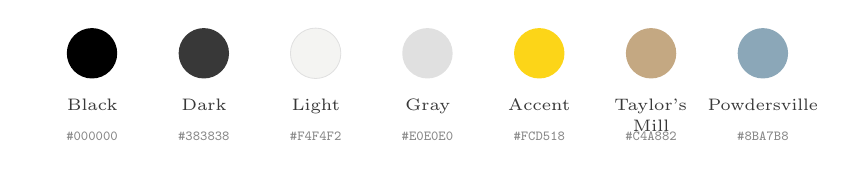
\begin{tikzpicture}
  \def\swatchspacing{1.42}
  \def\swatchradius{0.32}
  % Color data: name, hex, color
  \foreach \name/\hex/\col [count=\i from 0] in {
    Black/\#000000/wwsBlack,
    Dark/\#383838/wwsDark,
    Light/\#F4F4F2/wwsLight,
    Gray/\#E0E0E0/wwsGray,
    Accent/\#FCD518/wwsAccent,
    {Taylor's Mill}/\#C4A882/wwsTaylors,
    {Powdersville}/\#8BA7B8/wwsPowders%
  }{
    \pgfmathsetmacro{\xpos}{\i * \swatchspacing}
    % Swatch circle
    \ifnum\i=2
      % Light swatch needs a border
      \fill[\col] (\xpos,0) circle (\swatchradius);
      \draw[wwsGray, line width=0.3pt] (\xpos,0) circle (\swatchradius);
    \else
      \fill[\col] (\xpos,0) circle (\swatchradius);
    \fi
    % Name label
    \node[below, font=\interfont\fontsize{6}{7.5}\selectfont, text=wwsDark, text width=1.4cm, align=center] at (\xpos,-0.46) {\name};
    % Hex label
    \node[below, font=\interfont\fontsize{5.5}{7}\selectfont, text=wwsDark!60] at (\xpos,-0.88) {\texttt{\hex}};
  }
\end{tikzpicture}
\end{center}

% ════════════════════════════════════════════════════════════════
% TYPOGRAPHY
% ════════════════════════════════════════════════════════════════
\sheetsection{Typography}

\begin{multicols}{2}

% Cormorant Garamond
{\fontsize{20}{22}\selectfont\cormorantlight Cormorant Garamond}\\[2pt]
{\interfont\fontsize{6.5}{8}\selectfont\color{wwsDark!60} HEADINGS \enspace\textbar\enspace DISPLAY \enspace\textbar\enspace PULL QUOTES}

\vspace{4pt}
\begin{tabular}{@{}ll@{}}
{\cormorantlight\fontsize{11}{13}\selectfont Light 300 Specimen} &
  {\interfont\fontsize{6}{8}\selectfont\color{wwsDark!50} wght 300}\\[2pt]
{\fontsize{11}{13}\selectfont Regular 400 Specimen} &
  {\interfont\fontsize{6}{8}\selectfont\color{wwsDark!50} wght 400}\\[2pt]
{\cormorantsemibold\fontsize{11}{13}\selectfont SemiBold 600 Specimen} &
  {\interfont\fontsize{6}{8}\selectfont\color{wwsDark!50} wght 600}\\
\end{tabular}

\columnbreak

% Inter
{\interfont\fontsize{16}{18}\selectfont\addfontfeatures{RawFeature={+axis={wght=300}}} Inter}\\[2pt]
{\interfont\fontsize{6.5}{8}\selectfont\color{wwsDark!60} BODY \enspace\textbar\enspace UI \enspace\textbar\enspace NAVIGATION}

\vspace{4pt}
\begin{tabular}{@{}ll@{}}
{\interlight\fontsize{9}{11}\selectfont Light 300 Specimen} &
  {\interfont\fontsize{6}{8}\selectfont\color{wwsDark!50} wght 300}\\[2pt]
{\interfont\fontsize{9}{11}\selectfont Regular 400 Specimen} &
  {\interfont\fontsize{6}{8}\selectfont\color{wwsDark!50} wght 400}\\[2pt]
{\intermedium\fontsize{9}{11}\selectfont Medium 500 Specimen} &
  {\interfont\fontsize{6}{8}\selectfont\color{wwsDark!50} wght 500}\\[2pt]
{\intersemibold\fontsize{9}{11}\selectfont SemiBold 600 Specimen} &
  {\interfont\fontsize{6}{8}\selectfont\color{wwsDark!50} wght 600}\\
\end{tabular}

\end{multicols}

% ════════════════════════════════════════════════════════════════
% LOCATION IDENTITY
% ════════════════════════════════════════════════════════════════
\sheetsection{Location Identity}

\begin{minipage}[t]{0.48\linewidth}
  % Taylor's Mill panel
  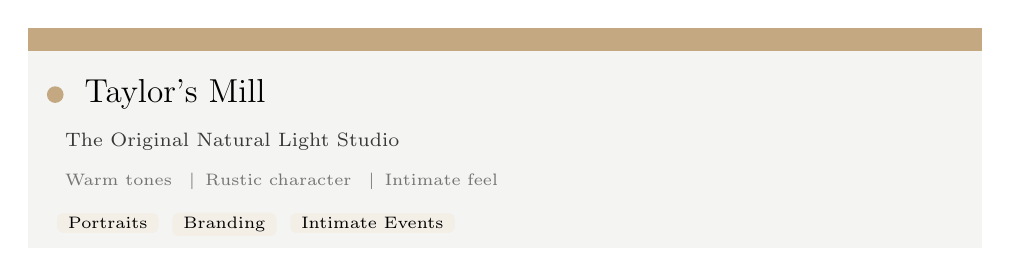
\begin{tikzpicture}
    \fill[wwsLight] (0,0) rectangle (\linewidth,2.8cm);
    % Color bar at top
    \fill[wwsTaylors] (0,2.5cm) rectangle (\linewidth,2.8cm);
    % Accent dot
    \fill[wwsTaylors] (0.35cm,1.95cm) circle (3pt);
    % Text
    \node[right, font=\cormorantsemibold\fontsize{13}{15}\selectfont, text=wwsBlack]
      at (0.6cm,1.95cm) {Taylor's Mill};
    \node[right, font=\interfont\fontsize{7.5}{9}\selectfont, text=wwsDark]
      at (0.35cm,1.35cm) {The Original Natural Light Studio};
    \node[right, font=\interfont\fontsize{6.5}{8}\selectfont, text=wwsDark!70]
      at (0.35cm,0.85cm) {Warm tones \enspace\textbar\enspace Rustic character \enspace\textbar\enspace Intimate feel};
    % Tags
    \node[right] at (0.25cm,0.3cm) {%
      \tag[wwsTaylors]{Portraits}\enspace
      \tag[wwsTaylors]{Branding}\enspace
      \tag[wwsTaylors]{Intimate Events}%
    };
  \end{tikzpicture}
\end{minipage}%
\hfill
\begin{minipage}[t]{0.48\linewidth}
  % Powdersville panel
  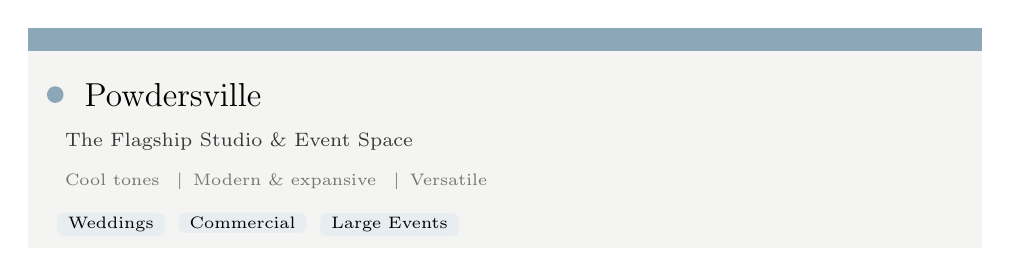
\begin{tikzpicture}
    \fill[wwsLight] (0,0) rectangle (\linewidth,2.8cm);
    % Color bar at top
    \fill[wwsPowders] (0,2.5cm) rectangle (\linewidth,2.8cm);
    % Accent dot
    \fill[wwsPowders] (0.35cm,1.95cm) circle (3pt);
    % Text
    \node[right, font=\cormorantsemibold\fontsize{13}{15}\selectfont, text=wwsBlack]
      at (0.6cm,1.95cm) {Powdersville};
    \node[right, font=\interfont\fontsize{7.5}{9}\selectfont, text=wwsDark]
      at (0.35cm,1.35cm) {The Flagship Studio \& Event Space};
    \node[right, font=\interfont\fontsize{6.5}{8}\selectfont, text=wwsDark!70]
      at (0.35cm,0.85cm) {Cool tones \enspace\textbar\enspace Modern \& expansive \enspace\textbar\enspace Versatile};
    % Tags
    \node[right] at (0.25cm,0.3cm) {%
      \tag[wwsPowders]{Weddings}\enspace
      \tag[wwsPowders]{Commercial}\enspace
      \tag[wwsPowders]{Large Events}%
    };
  \end{tikzpicture}
\end{minipage}

% ════════════════════════════════════════════════════════════════
% DESIGN PRINCIPLES
% ════════════════════════════════════════════════════════════════
\sheetsection{Design Principles}

\newlength{\princwidth}
\setlength{\princwidth}{0.185\linewidth}
\newcommand{\principle}[2]{%
  \begin{minipage}[t]{\princwidth}%
    \raggedright
    {\intersemibold\fontsize{7}{9}\selectfont #1}\\[1.5pt]%
    {\interfont\fontsize{6.5}{8.5}\selectfont\color{wwsDark} #2}%
  \end{minipage}%
}

\noindent
\principle{Photography First}{Imagery leads, UI recedes. Full-bleed heroes, minimal overlays.}%
\hfill
\principle{Location-Aware}{Nav adapts color and content per studio. Visitors always know where they are.}%
\hfill
\principle{Warm vs.\ Cool}{Taylor's Mill = earthy gold; Powdersville = slate blue. Never mix them.}%
\hfill
\principle{Generous Space}{Let the work breathe. Padding over packing. White\-space is intentional.}%
\hfill
\principle{Content First}{No gratuitous animations. Subtle transitions only where they aid comprehension.}

% ════════════════════════════════════════════════════════════════
% UI PATTERNS
% ════════════════════════════════════════════════════════════════
\sheetsection{UI Patterns}

\begin{multicols}{3}

% Buttons
{\intersemibold\fontsize{7}{9}\selectfont Buttons}\par\vspace{2pt}
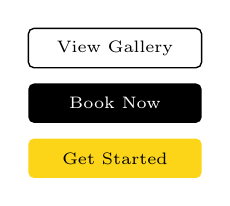
\begin{tikzpicture}
  % Outline button
  \draw[wwsBlack, line width=0.5pt, rounded corners=2pt] (0,0) rectangle (2.2cm,0.5cm);
  \node[font=\interfont\fontsize{6}{8}\selectfont] at (1.1cm,0.25cm) {View Gallery};
  % Solid button
  \fill[wwsBlack, rounded corners=2pt] (0,-0.7cm) rectangle (2.2cm,-0.2cm);
  \node[font=\interfont\fontsize{6}{8}\selectfont, text=white] at (1.1cm,-0.45cm) {Book Now};
  % Accent button
  \fill[wwsAccent, rounded corners=2pt] (0,-1.4cm) rectangle (2.2cm,-0.9cm);
  \node[font=\intersemibold\fontsize{6}{8}\selectfont, text=wwsBlack] at (1.1cm,-1.15cm) {Get Started};
\end{tikzpicture}

\columnbreak

% Cards
{\intersemibold\fontsize{7}{9}\selectfont Cards \& Content}\par\vspace{2pt}
{\interfont\fontsize{6.5}{8.5}\selectfont
  Flat cards on \texttt{\#F4F4F2} bg\par
  No drop shadows\par
  1px \texttt{\#E0E0E0} border optional\par
  16px padding, 8px gap\par
  Image ratio: 3\kern0.5pt:\kern0.5pt{}2 or 16\kern0.5pt:\kern0.5pt{}9\par
}

\columnbreak

% Nav & Spacing
{\intersemibold\fontsize{7}{9}\selectfont Navigation \& Spacing}\par\vspace{2pt}
{\interfont\fontsize{6.5}{8.5}\selectfont
  Fixed top nav, white bg\par
  Logo left, links right\par
  Location indicator dot\par
  Section padding: 80\,\textendash\,120px\par
  Max content width: 1280px\par
  Mobile: hamburger menu\par
}

\end{multicols}

\vfill
{\color{wwsGray}\rule{\linewidth}{0.4pt}}
{\interfont\fontsize{6}{8}\selectfont\color{wwsDark!50} WhiteWall Studios \enspace\textbar\enspace Design System v1.0 \enspace\textbar\enspace March 2026 \enspace\textbar\enspace Prepared by Andrew Smith}

\end{document}
